\section{Environmental Permit Application Process}
\label{sec:environmental-permit-application-process}
In this section, methodology proposed in this thesis study will be applied on the \textit{Environmental Permit Application Process} dataset \cite{coselog-data} and evaluation results will be presented with a similar approach above. Since this dataset consists of real-life event logs, preprocessing is undertaken prior to start analysis. Incomplete traces, which started but not ended in the time frame of log collection, and exceptional cases are removed from event logs with the help of ProM log visualization tools with a similar approach in \cite{buijs2014flexible}. Statistical information about the dataset that is used in this section can be summarized in Table~\ref{table:coselog-process-summary}.

%\caption{Statistical summary of Environmental Permit Application Process dataset}
%\label{table:coselog-process-summary}
 \begin{table}[]
\centering
\caption{Statistical summary of Environmental Permit Application Process dataset}
\label{table:coselog-process-summary}
\begin{tabular}{lccc}
\hline
                       & {\bf Cases} & {\bf Events} & {\bf Percentage} \\ \hline
{\bf Municipality \#1} & 54          & 131          & 6.1 \%           \\ \hline
{\bf Municipality \#2} & 302         & 586          & 27.3 \%          \\ \hline
{\bf Municipality \#3} & 37          & 73           & 3.4 \%           \\ \hline
{\bf Municipality \#4} & 340         & 507          & 23.7 \%          \\ \hline
{\bf Municipality \#5} & 481         & 845          & 39.4 \%          \\
{\bf Total}            & {\bf 1214}  & {\bf 2142}   & {\bf }           \\ \hline
\end{tabular}
\end{table}

As shown in Table~\ref{table:coselog-process-summary}, total of 1214 cases and 2142 events included in this dataset with a variable distribution between event logs of municipalities. In the following sections, these municipalities will be used as organizational logs and the methodology presented in this thesis study will be applied.

\subsection{Methodology Stages}
\label{sec:coselog-methodology}
In \textit{Process Model Mining} stage, event logs of each municipality in the dataset are used as organizational event logs and they are used to mine process models. Considering preprocessing is undertaken on the event logs, noise threshold in \textit{Inductive Miner} is set to a low value of 10\% to achieve a higher fitness. 

Appropriateness and fitness evaluation metrics are summarized in Table~\ref{table:coselog-wabo-process-model-mining} and it can be seen that each event log is successful in terms of representing reality with high fitness values. However, some of the process models like Municipality \#5 and \#4 resulted with low appropriateness values. Process models for each event log are visualized with a detail simplification based on number of activities and paths in Figure~\ref{fig:coselog-wabo-process-models} and it can be seen that low appropriateness values resulted with complicated process models that are difficult to analyze visually. Detail simplification is only used for visualization and it draws the mainstream process flows instead of whole set of paths and activities. It should be kept in mind that actual process models are 10 to 20 times more complicated in terms of number of activities and paths than the ones presented in Figure~\ref{fig:coselog-wabo-process-models}. 
%\caption{Process Model Mining Evaluation of Environmental Permit Application Process Dataset}
%\label{table:coselog-wabo-process-model-mining}
\begin{table}[]
\centering
\caption{Process Model Mining Evaluation of Environmental Permit Application Process Dataset}
\label{table:coselog-wabo-process-model-mining}
\begin{tabular}{lcccc}
\hline
 & {\bf Fitness} & {\bf \begin{tabular}[c]{@{}c@{}}Structural\\Appropriateness\end{tabular}} & {\bf \begin{tabular}[c]{@{}c@{}}Behavioral\\Appropriateness\end{tabular}} & {\bf \begin{tabular}[c]{@{}c@{}}Average\\Appropriateness\end{tabular}} \\ \hline
{\bf Municipality \#1} & 86 \% & 97.5 \% & 54.4 \% & 76 \% \\ \hline
{\bf Municipality \#2} & 100 \% & 100 \% & 100 \% & 100 \% \\ \hline
{\bf Municipality \#3} & 92.3 \% & 71.1 \% & 67.2 \% & 69.1 \% \\ \hline
{\bf Municipality \#4} & 96.8 \% & 65.7 \% & 64 \% & 64.9 \% \\ \hline
{\bf Municipality \#5} & 94.5 \% & 58.8 \% & 39.7 \% & 49.3 \% \\ \hline
{\bf Average} & {\bf 93.9 \%} & {\bf 78.6 \%} & {\bf 65.1 \%} & {\bf 71.9 \%} \\ \hline
\end{tabular}
\end{table}

\begin{figure}
\centering
  \begin{subfigure}[t]{.4\textwidth}
    \centering
    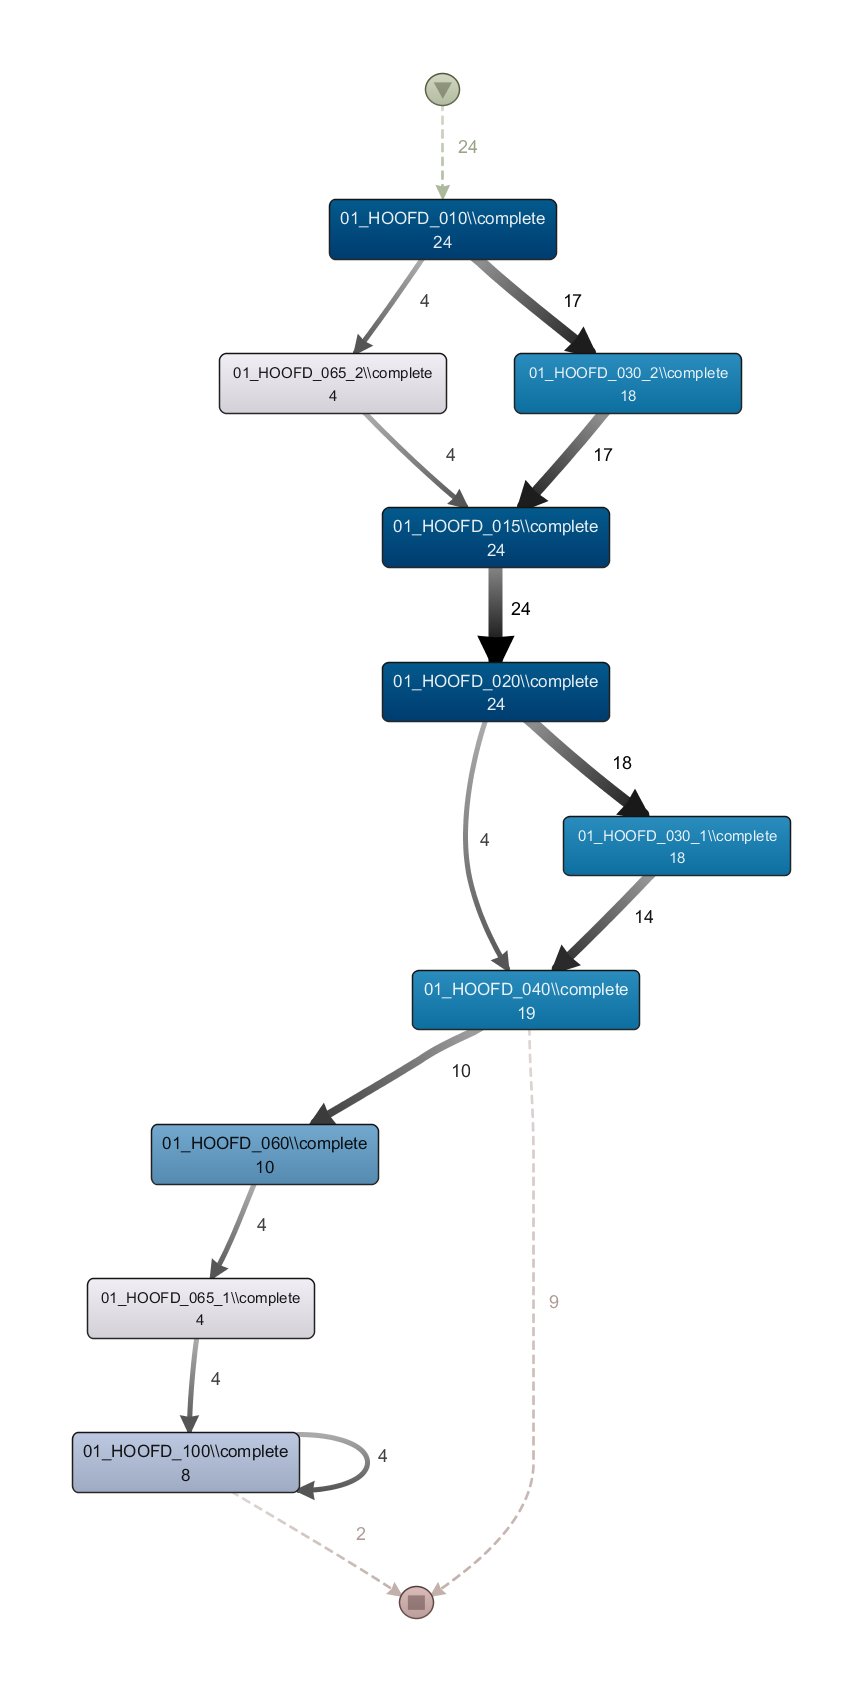
\includegraphics[width=1\linewidth]{5_results_discussions/coselog-wabo/coselog-wabo-1-simplified}
    \caption{Municipality \#1}
    \label{fig:coselog-wabo-process-models-simplified-1}
  \end{subfigure}%
  \begin{subfigure}[t]{.2\textwidth}
    \centering
    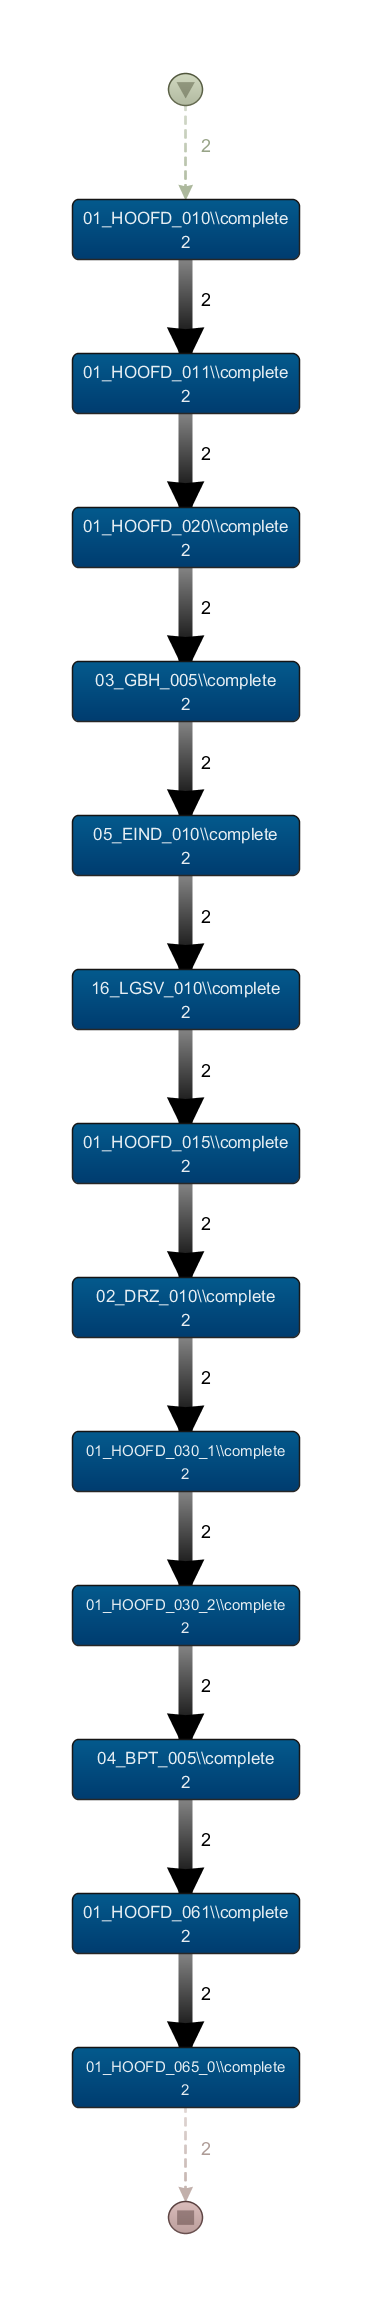
\includegraphics[width=.6\linewidth]{5_results_discussions/coselog-wabo/coselog-wabo-2-simplified}
    \caption{Municipality \#2}
    \label{fig:coselog-wabo-process-models-simplified-2}
  \end{subfigure} 
  \begin{subfigure}[t]{.3\textwidth}
    \centering
        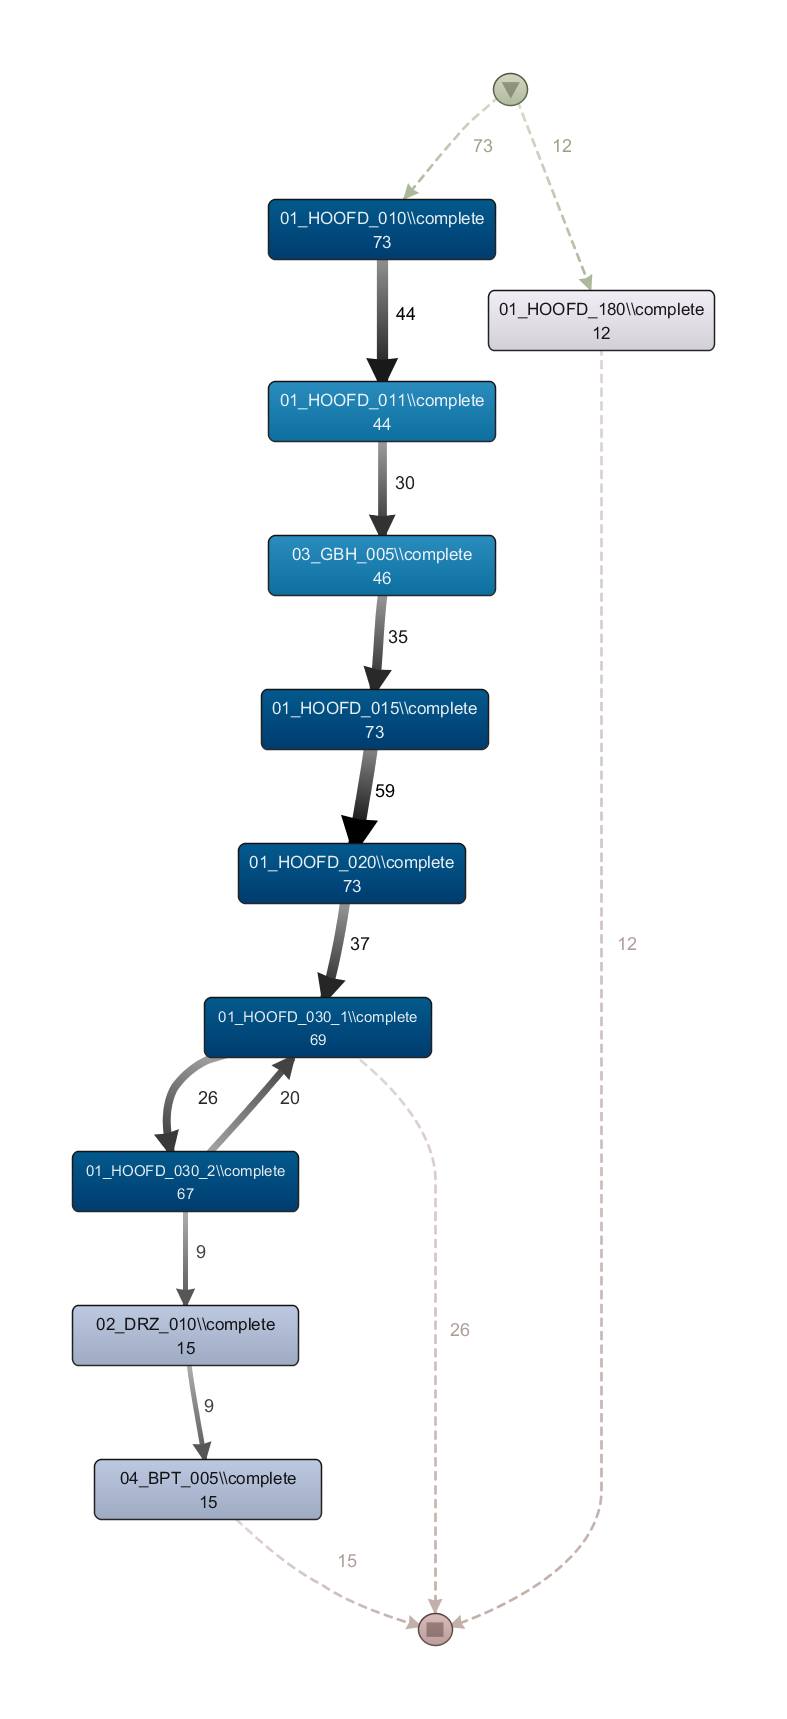
\includegraphics[width=1\linewidth]{5_results_discussions/coselog-wabo/coselog-wabo-3-simplified}
    \caption{Municipality \#3}
    \label{fig:coselog-wabo-process-models-simplified-3}
  \end{subfigure} 
  \begin{subfigure}[t]{.4\textwidth}
    \centering
        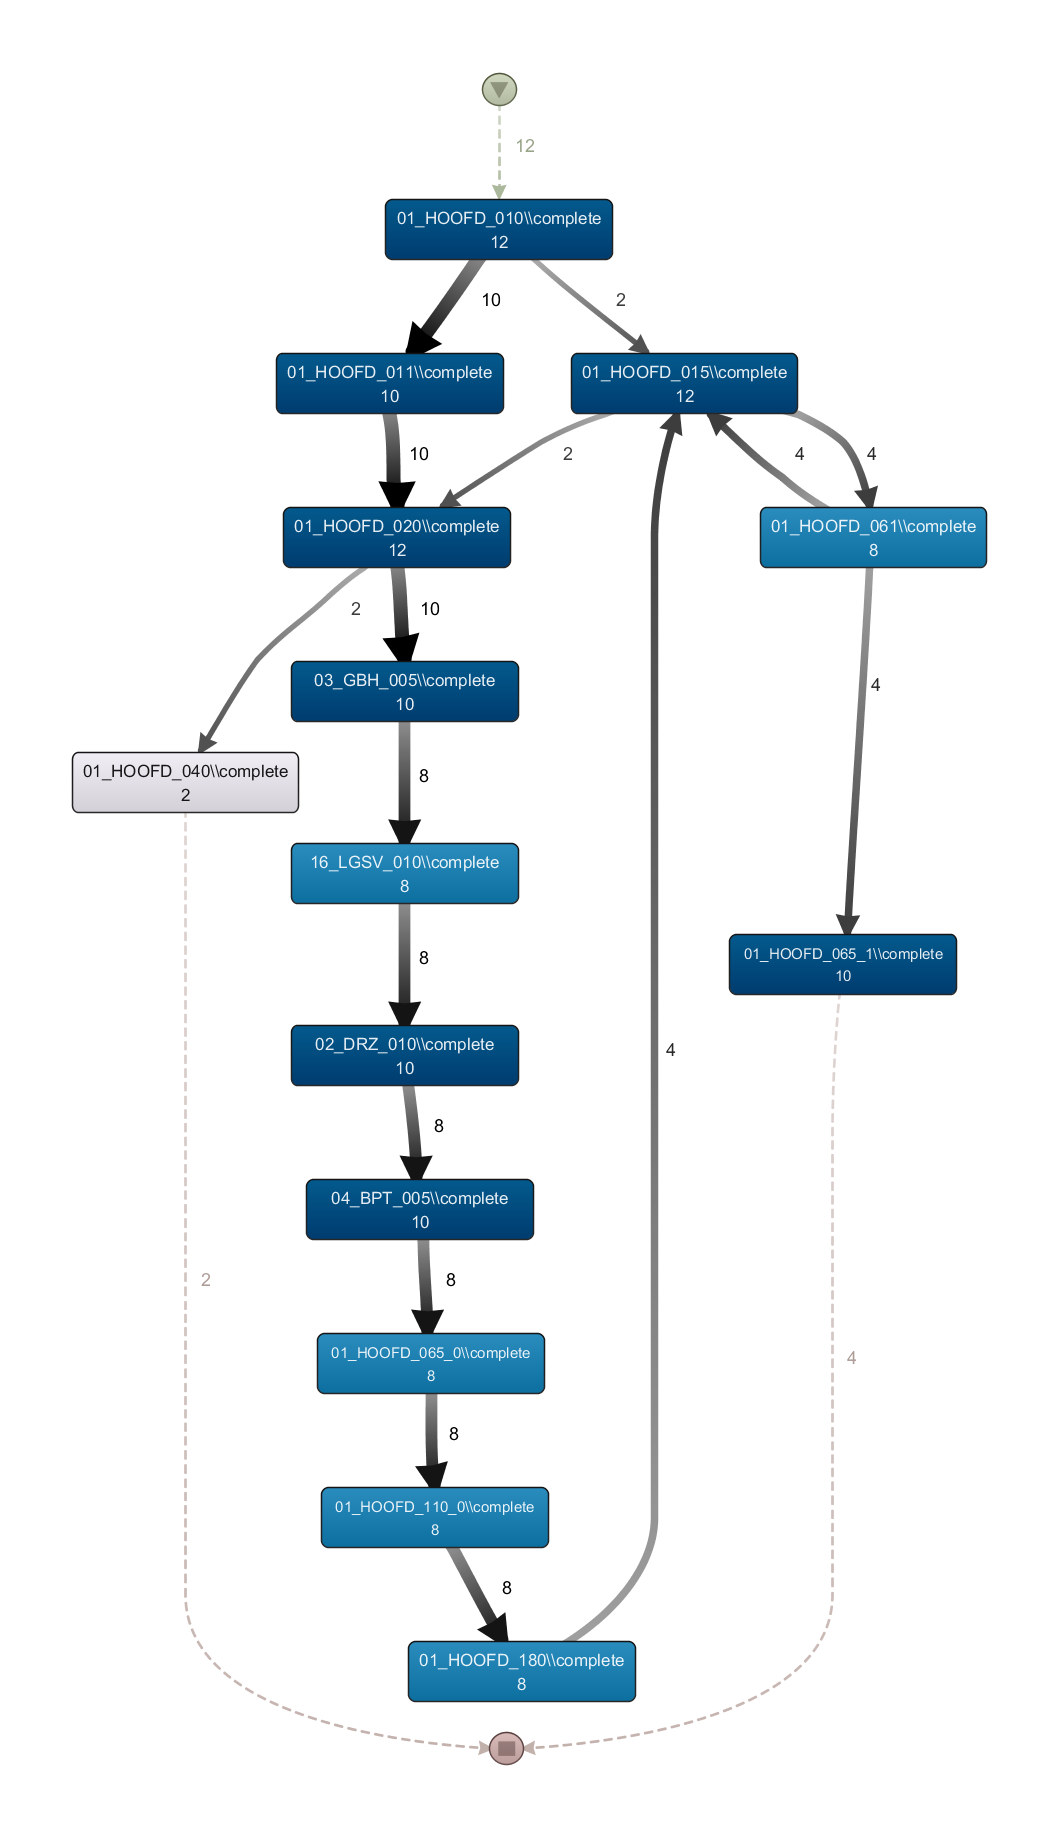
\includegraphics[width=1\linewidth]{5_results_discussions/coselog-wabo/coselog-wabo-4-simplified}
    \caption{Municipality \#4}
    \label{fig:coselog-wabo-process-models-simplified-4}
  \end{subfigure}
    \begin{subfigure}[t]{.4\textwidth}
    \centering
        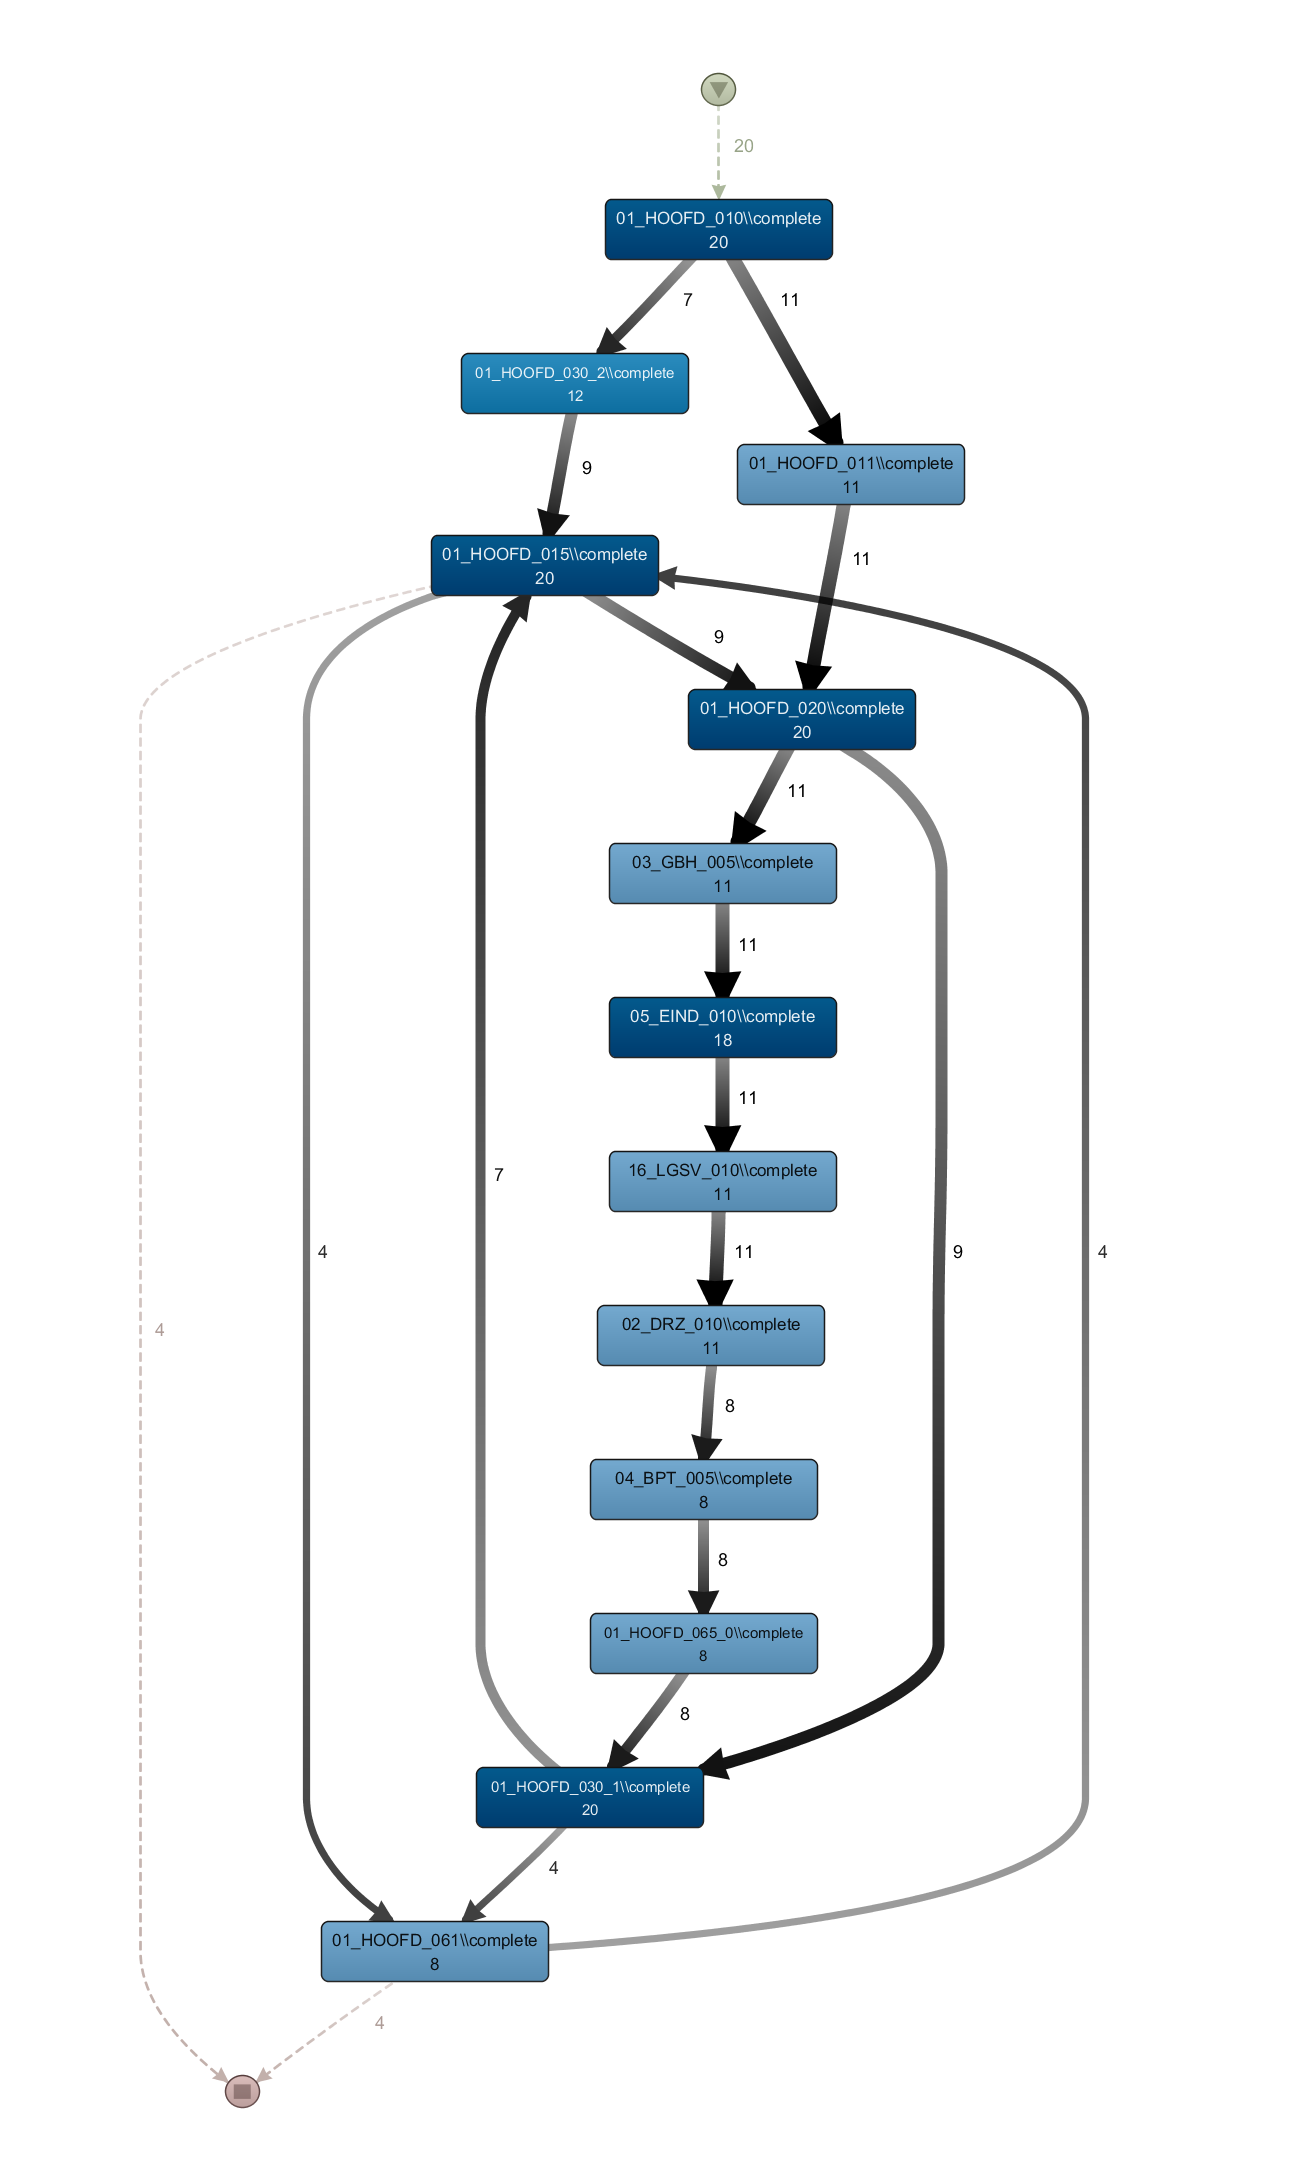
\includegraphics[width=1\linewidth]{5_results_discussions/coselog-wabo/coselog-wabo-5-simplified}
    \caption{Municipality \#5}
    \label{fig:coselog-wabo-process-models-simplified-5}
  \end{subfigure}%
\caption{Process models of Environmental Permit Application Process Dataset}
\label{fig:coselog-wabo-process-models}
\end{figure} 



In \textit{Performance Indicator Analysis} stage, alignment costs are calculated over replay of event logs on process models. As presented in the Table~\ref{table:coselog-wabo-replay}, as appropriateness and fitness decrease alignment costs increase for the municipalities. This indicates the fact that both process model mining stage and replay stage is in conformity and performance indicators calculated over replay are acceptable.
%\caption{Replay Evaluation of Environmental Permit Application Process Dataset}
%\label{table:coselog-wabo-replay}
\begin{table}[]
\centering
\caption{Replay Evaluation of Environmental Permit Application Process Dataset}
\label{table:coselog-wabo-replay}
\begin{tabular}{lccc}
\hline
 & {\bf Fitness} & {\bf Average Appropriateness} & {\bf Alignment Cost} \\ \hline
{\bf Municipality \#1} & 86 \% & 76 \% & 173.2 \\ \hline
{\bf Municipality \#2} & 100 \% & 100 \% & 0 \\ \hline
{\bf Municipality \#3} & 92,3 \% & 69,1 \% & 332.3 \\ \hline
{\bf Municipality \#4} & 96,8 \% & 64,9 \% & 9,1 \\ \hline
{\bf Municipality \#5} & 94,5 \% & 49,3 \% & 35.8 \\ \hline
\end{tabular}
\end{table}

After calculating the performance indicators, municipalities are clustered based on these values and this stage is evaluated by the within-SSE values for different number of clusters as plotted in Figure~\ref{fig:coselog-wabo-cluster-sse-plot}. In order to avoid overfitting of clusters, number of clusters, \textit{k}, is selected to be 2 for this dataset for further analysis. For two clusters, Municipality \#1 is located in one cluster where municipalities \#2, \#3, \#4 and \#5 are grouped into to other cluster.
\begin{figure}
	\centering
	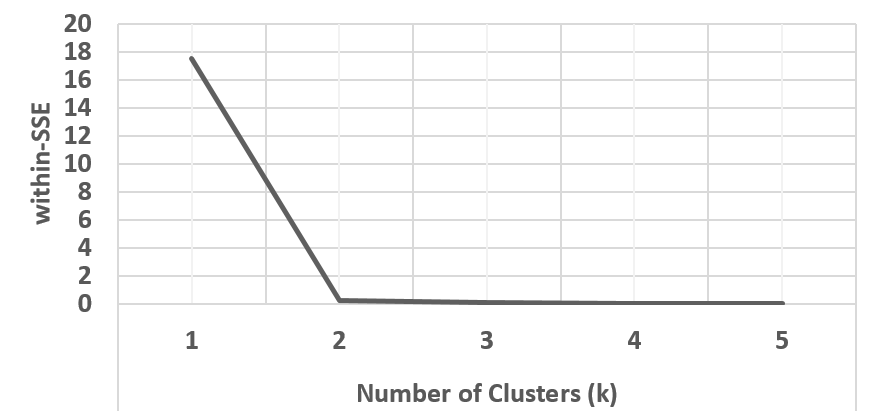
\includegraphics[width=.7\textwidth]{5_results_discussions/coselog-wabo/cluster-sse-plot}
	\caption{Number of Clusters vs. within-SSE for Environmental Permit Application Process Dataset}
  \label{fig:coselog-wabo-cluster-sse-plot}
\end{figure}

In \textit{Mismatch Pattern Analysis} stage, number of mismatch patterns are analyzed with the \textit{graph-edit similarity} between each two municipality. In order to check correlation between \textit{graph-edit similarity} and number of mismatch patterns, data is plotted in Figure~\ref{fig:coselog-wabo-pattern-analysis-results}. When the plot is checked, it can be seen that as the similarity between process models of municipalities increases, number of mismatch patterns decreases on most of the cases. When further analyzed, it can be seen that Municipalities \#4 and \#5, which have significantly more complex process model compared to others, fails in spotting mismatch patterns according to \textit{graph-edit similarity}.
\begin{figure}
	\centering
	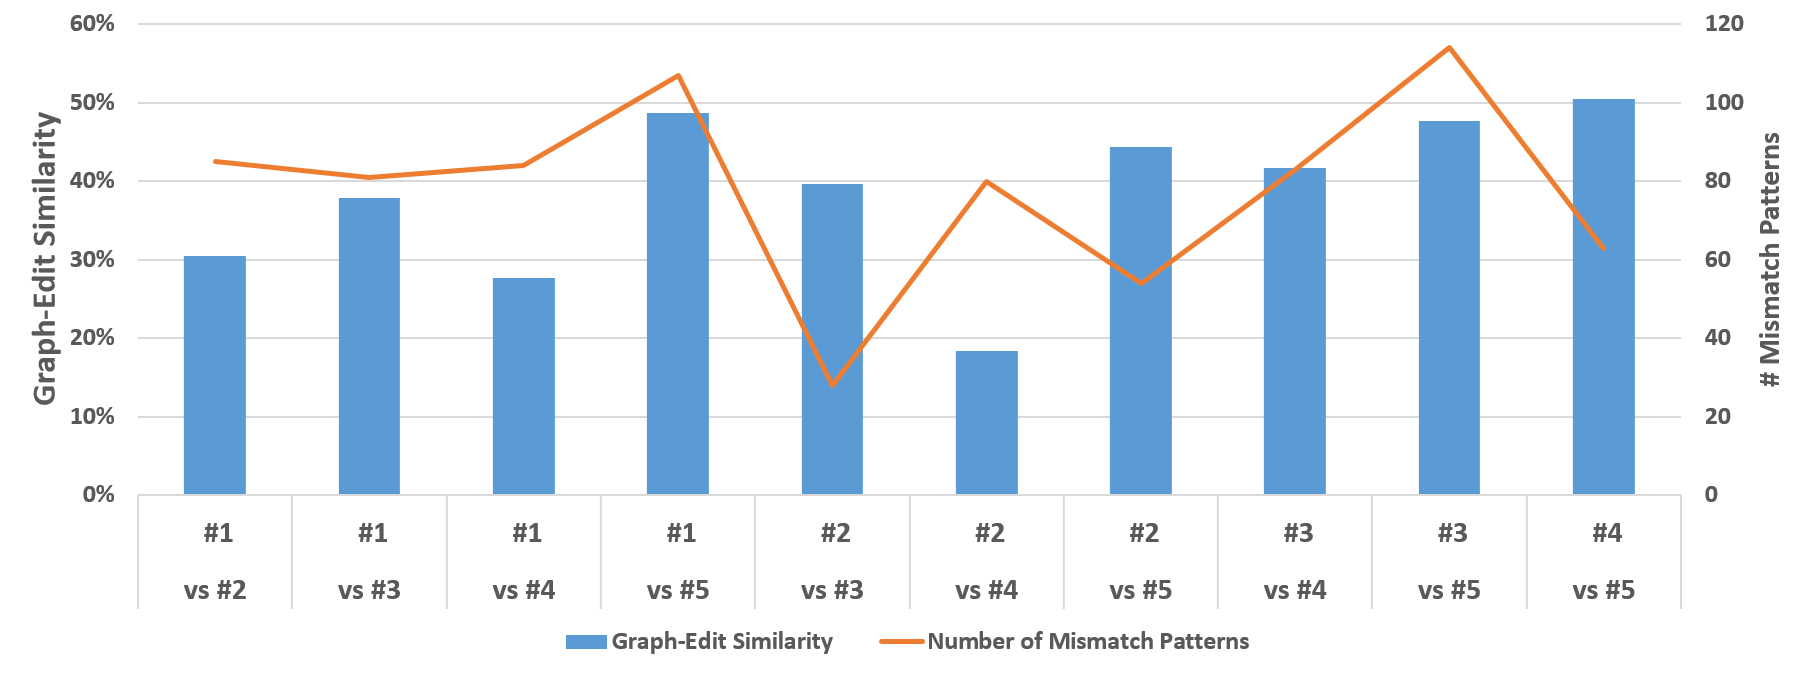
\includegraphics[width=\textwidth]{5_results_discussions/coselog-wabo/mismatch-pattern-analysis-results}
	\caption{Mismatch Patterns vs. Graph-Edit Similarity for Environmental Permit Application Process Dataset}
  \label{fig:coselog-wabo-mismatch-pattern-analysis-results}
\end{figure}
When the mismatch patterns are analyzed according to their types as plotted in Figure~\ref{fig:coselog-wabo-mismatch-pattern-types}, mostly \textit{Skipped Activity} pattern is spotted. Following these, \textit{Different Dependencies} and \textit{Additional Dependencies} are spotted between process models of municipalities. Unlike the synthetic dataset, there are on average of 78 mismatch patterns are spotted for process models of municipalities. Unfortunately, \textit{Refined Activity} pattern analyzers could not be applied on this dataset since activity names are not provided in this dataset and instead of activity codes without any semantic meaning are used. Since the \textit{Refined Activity} pattern in this study is based on the difference between labels, they are eliminated in the analysis of this dataset.
\begin{figure}
	\centering
	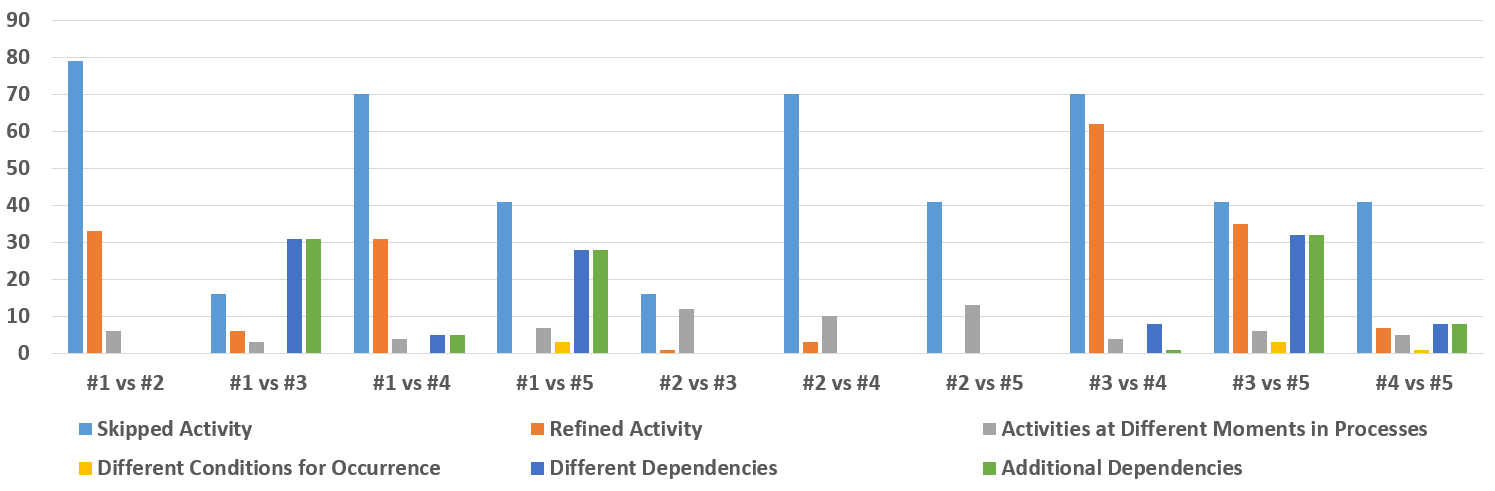
\includegraphics[width=\textwidth]{5_results_discussions/coselog-wabo/mismatch-pattern-types}
	\caption{Mismatch Pattern Types for Environmental Permit Application Process Dataset}
  \label{fig:coselog-wabo-mismatch-pattern-types}
\end{figure} 

In \textit{Recommendation Generation} stage, an organization and performance difference threshold is selected as analysis input likewise the previous dataset. For different threshold values, number of performance indicators that are performing better for the selected organization and spotted mismatch patterns are plotted in Figure~\ref{fig:coselog-wabo-recommendation-generation-analysis}. 
\begin{figure}
	\centering
	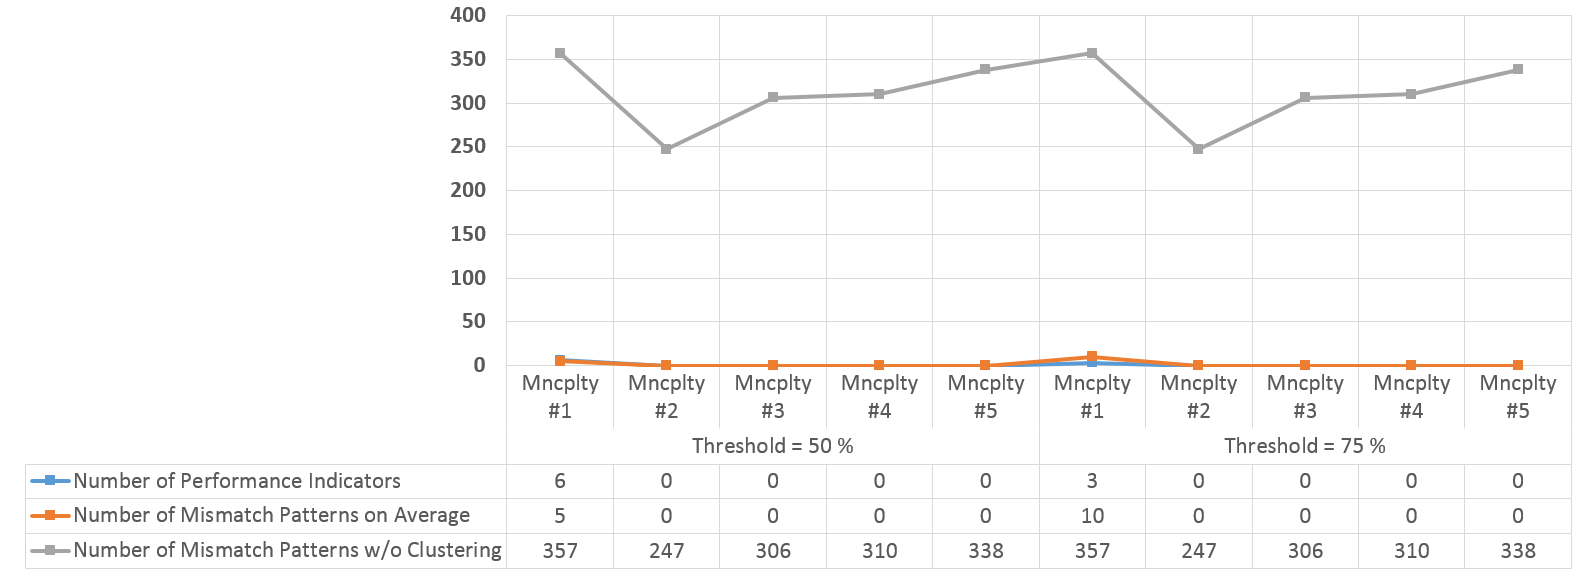
\includegraphics[width=\textwidth]{5_results_discussions/coselog-wabo/recommendation-generation-analysis}
	\caption{Recommendation Generation Analysis for Environmental Permit Application Process Dataset (2 Clusters)}
  \label{fig:coselog-wabo-recommendation-generation-analysis}
\end{figure}

In the analysis of Figure~\ref{fig:coselog-wabo-recommendation-generation-analysis}, it can be seen that only the cluster that the Municipality \#1 has the potential of learning from other cluster since it performs worse in performance indicators. For the threshold of 50\%, cluster of Municipality \#1 performs worse in 6 performance indicators and proposed approach lists total of 30 mismatch patterns. On the average it show 6 patterns to the user as the potential causes of performance improvement. With the same approach, cluster of Municipality \#1 performs worse in 3 indicators with the difference of 75 \% and on average 10 mismatch patterns are listed for each performance indicator. When it is compared to the total mismatch patterns of Municipality #1, which is 357, proposed approach helps significantly to the user for focusing performance improvement.

Since selecting number of clusters as 2 did not yield high learning potential for performance improvement, analysis is repeated with selecting number of clusters as 3. When three clusters are created, Municipality \#1 is located in the first cluster; Municipality \#2 and \#4 are located in the second cluster; and Municipality \#3 and \#5 are grouped in to the last cluster. For these clusters analysis is repeated for threshold of 25 \%, 50 \% and 75 \%, and as plotted in Figure~\ref{fig:coselog-wabo-recommendation-generation-analysis-k3}, in addition to Municipality \#1, now Municipality \#3 and \#5 have the learning potential from other clusters. However, Municipality \#2 and \#4 performs better in all performance indicators which yielded no mismatch pattern analysis data for them. Increasing cluster sizes in this analysis shows that organizations can learn more from each other but it has the potential danger of overfitting to other organizations process model. 
\begin{figure}
	\centering
	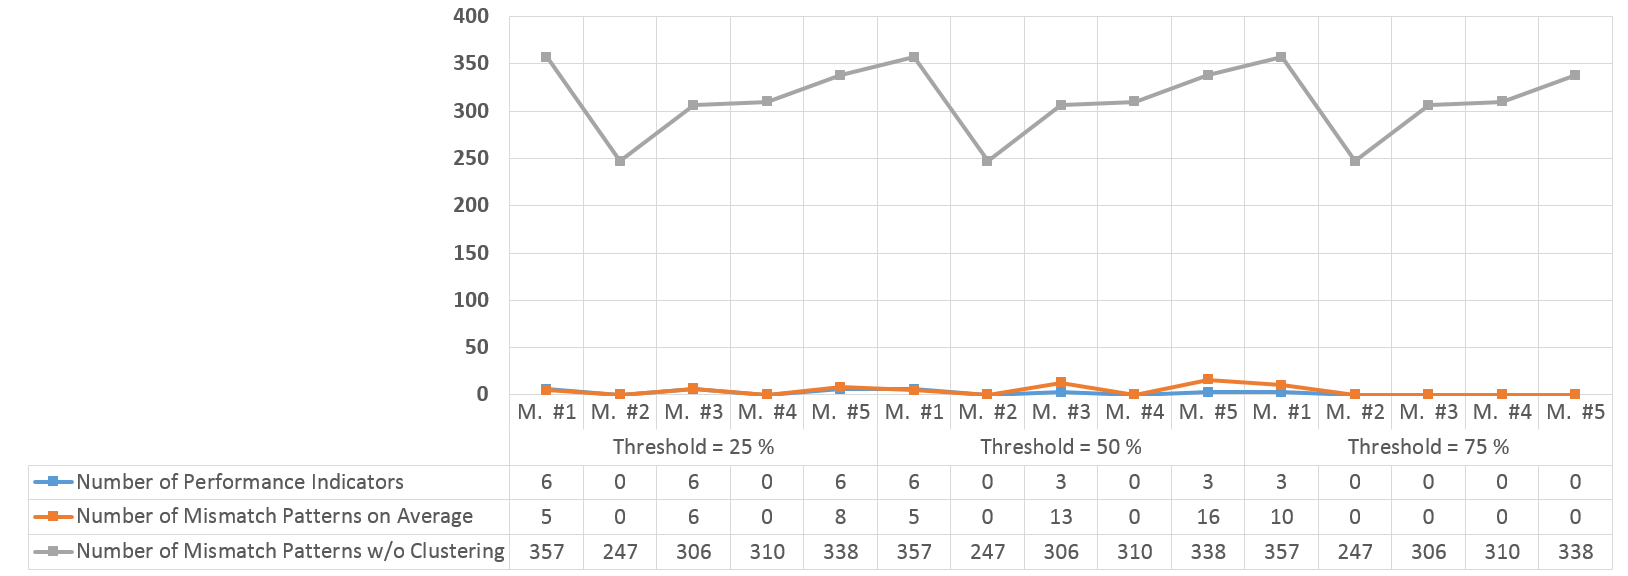
\includegraphics[width=\textwidth]{5_results_discussions/coselog-wabo/recommendation-generation-analysis-k3}
	\caption{Recommendation Generation Analysis for Environmental Permit Application Process Dataset (3 Clusters)}
  \label{fig:coselog-wabo-recommendation-generation-analysis-k3}
\end{figure}

\subsection{Discussions}
\label{sec:coselog-discussions}
\todo{write}
%evaluation metric'ler ve stage'lerin özetini geç
%çıkan sonuçların visual değerlendirmesini yap
